\subsection{The architecture}
\label{sec:overview:libos:arch}

%Recent library OSes~\cite{porter11drawbridge,unikernels,baumann13bascule,osv}
%are designed for security and efficiency, but are limited to single-process applications.
%The security isolation of \liboses{} derives from 
%limited, explicit data sharing and 
%a narrow host interface.  
A \libos{} typically executes in either a paravirtual VM~\cite{unikernels,osv}
% \daniela{I would have the use of a VM as a discussion topic in the end of the paper.}, 
or an OS process, called a \emph{Picoprocess}~\cite{porter11drawbridge,baumann13bascule}, with interfaces restricted to a narrowed host ABI.
%The host ABI heavily restrict effects outside of the application's address space
%as a result, applications in a \picoproc{} have very little opportunity to interfere with each other,
%yielding security isolation comparable to a VM.
The library OS deduplicates features for hardware management in both the guest and host kernels.
\graphene{} executes within a \picoproc{} (Figure~\ref{fig:overview:arch}),
which includes an {\em unmodified} application and its supporting libraries, both of which run on a library OS instance.
The \libos{} is implemented over the kernel ABI designed to expose very generic abstractions that can be easily implemented on any host OS.
%Although the \graphene{} prototype  host kernel is Linux, 
%we adapt a host ABI from Drawbridge/Bascule,
%which has been previously implemented on Windows, Hyper-V, and Barrelfish~\cite{porter11drawbridge,baumann13bascule,baumann09barrelfish}.
%The \graphene{} host ABI is
% summarized in Table~\ref{tab:abi} and discussed in more detail in \S\ref{sec:linux:pal}\fixmedp{if not cut...}.  
%which exposes only tens of simple host calls. \daniela{briefly define \picoproc{}: A \picoproc{} is unmodified application code running with a \libos{}.}


\begin{figure}[t]
\centering
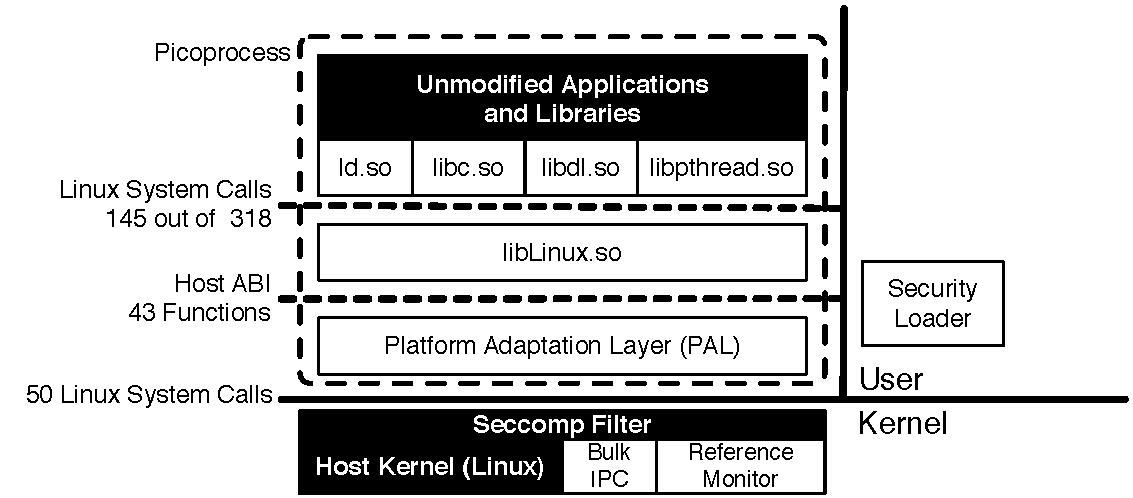
\includegraphics[width=\textwidth]{arch.pdf}
\caption{Building blocks of \graphene{}.  Black components are unmodified.
We modify the four lowest application libraries on Linux:
{\tt ld.so} (the ELF linker and loader),
{\tt libdl.so} (the dynamic library linker),
{\tt libc.so} (standard library C),
and {\tt libpthread.so} (standard threading library), that issue Linux system calls as function calls directly to {\tt libLinux.so}.
Graphene implements the Linux system calls using a variant of the Drawbridge ABI, which is provided by the platform adaption layer (PAL).
A trusted reference monitor that ensures \libos{} isolation is implemented as a kernel module. Another small module is added for fast bulk IPC, but it is optional for hosts other than Linux.}
\label{fig:overview:arch}
\end{figure}


The library OS shows that the host ABI is sufficient to implement the guest OS functionality.
As an example of this layering, consider the heap memory management abstraction. Linux provides applications with a data segment---a legacy abstraction dating back to original Unix and the era of segmented memory. The primary thread's stack is at one end of the data segment, and the heap is at another.  The heap grows up (extended by \syscall{brk}) and the stack grows down until they meet in the middle.
In contrast, the host ABI provides only simple abstraction that allocate, deallocate, or protect regions of virtual memory.
This clean division of labor encapsulates idiosyncratic abstractions
in the library OS.


%These interfaces are host-independent \daniela{OS or kernel-independent}, as they tend to be very generic and easily
%implemented on any host OS kernel or VMM \daniela{postpone VMM for later}.

At a high level, these library OS designs
scoop the layer just below the system call table out of the OS kernel
and refactor this code as an application library.  
The driving insight is that there is a natural, functionally-narrow division point 
one layer below the system call table
in most OS kernels.
Unlike many OS interfaces, the host ABI generally minimize the amount of application state in the kernel, facilitating
migration: a library OS instance can programmatically read and modify its own OS state, copy the state to another instance, and the remote instancey OS can 
load a copy of this state into the OS---analogous to hardware registers.
A \picoproc{} may not modify another \picoproc{}'s OS state.



\subsection{Multi-process support}
\label{sec:overview:libos:multiproc}

A key design feature of Unix is that users compose simple utilities to create larger applications.  Thus, it is unsurprising that many popular applications for Unix or Linux require multiple processes---an essential feature missing from current library OS designs.
%This gap is filled by the \graphene{} \libos{}, which
%extends recent \liboses{} to support multi-process applications.
The underlying design challenge is minimally expanding a tightly-drawn isolation boundary without also exposing idiosyncratic kernel abstractions or re-duplicating mechanisms in both the host kernel and the library OS.

%requires a careful balance among the competing goals of 
%efficiency, host independence, and security isolation.
%The challenge, then, is minimal expansion of

%\vspace{5pt}
%\noindent {\bf Motivating Example.~}
For example, consider the process identifier (PID) namespace. In current, single-process library OSes, \syscall{getpid} could simply return a fixed value to each application.
This single-process design is isolated, but the library OS cannot run a shell script, which requires \syscall{fork}'ing and \syscall{exec}'ing multiple binaries, signaling, waiting, and other PID-based APIs.

\vspace{5pt}
\noindent{\bf Design Options.~}
%Multi-process support requires extensions to the host ABI of recent, single-process library OS designs. Because multi-process abstractions, such as signals or System V IPC, tend to be idiosyncratic, an essential problem is identifying a minimal, host-independent substrate upon which  to implement OS-specific abstractions.
There are two primary design options: (1) implement processes and scheduling in 
the library OS, and (2) treat each library OS instance as a process, and distribute the shared POSIX implementation across a collection of library OSes.
\graphene{} follows the second option, which imposes fewer host assumptions.
%, maximize flexibility in mapping processes to physical resources, and facilitate inter-process security policy enforcement. % as enforcing security policies on related processes.

Implementing processes
inside the library OS is also feasible using 
hardware MMU virtualization, similar to Dune~\cite{belay12dune},
but this reintroduces a duplicate scheduler and memory management.
Moreover, Intel and AMD have similar, but mutually incompatible MMU virtualization support,
which would complicate live migration across platforms.
None of these problems are insurmountable, and it would be interesting in future
work to compare both options.


In \graphene{}, multiple library OS instances in multiple picoprocesses collaborate to implement shared abstractions. The supported Linux abstractions include copy-on-write \syscall{fork}, signals, exit notification, and System V IPC semaphores and message queues.
For instance, when process A signals process B on \graphene{}, A's library OS instance issues a query to B's instance over a host RPC stream (similar to a Unix pipe), and B's instance then calls the appropriate signal handler.

%%% All collaborating \libos{} instances exchange messages as needed 
%%% to provide the application with a consistent view of 
%%% shared abstractions,
%%% such as


%\graphene{} approaches multi-processing by selectively replicating state and issuing remote procedure calls (RPCs) 
%%across multiple, collaborating
%library OS instances.
%Guests may work together to provide the unmodified multi-process application with
%coordination abstractions 

%Shared abstractions on \graphene{}'s are implemented outside of the host, ensuring  host OS independence.
% by implementing these
%shared abstractions entirely
%outside of the host kernel.
%Shared abstractions are implemented outside of the host.
%From the host kernel's perspective, 
\graphene{} implements all shared abstractions by cooperatively managing the abstraction states over RPC streams.
Single-process applications still service system calls from local state, and \graphene{}, includes optimizations to place state where it is most likely to be used, minimizing RPC overheads.
The host reference monitor can easily isolate picoprocesses by 
% \graphene{} design isolates \liboses{} by 
%requiring all coordination to use 
%explicit bytes streams \daniela{, pipe-like abstractions provided by the kernel. (suggestion: Reviewer  3)}.
%Security isolation is enforced
%by a kernel-level {\em reference monitor}, which can 
%disconnect or prevent creation of a
blocking all RPC messages, % between \liboses{} that should be isolated,
without the need to understand the library OS details or semantics of these abstractions.
In the PID example, only mutually-trusting picoprocesses can signal each other.
%if the reference monitor prevents creation of RPC streams
%across mutually untrusting \picoprocs{},
%the \liboses{} cannot exchange signals.

%%% \graphene{} is designed to 
%%% The \graphene{} design leverages a number of optimizations to service application system calls 
%%% from local state whenever possible, and to minimize message passing overheads otherwise
%%%  (\S\ref{sec:namespaces:insights}).
%%% Our experience is that starting with a local system call design and then extending it to share state is relatively straightforward,
%%% and introduces little-to-no overhead when the request can be serviced locally.


The \graphene{} library OS is designed to gracefully handle disconnection from other library OSes, facilitating dynamic application sandboxing.
RPC streams may be disconnected at any time by either the reference monitor or at the request of a library OS.
%Message streams may be severed externally, by the reference monitor, or 
%one guest may simply disconnect from others to isolate itself.
%An application may disconnect itself from the 
%Any \graphene{} application may dynamically detach from the confederation, 
%or a host-level sandbox may dynamically separate two guests by severing their communication channels.
When a picoprocess is disconnected, the library OS will handle the subsequent
divergence, %and the library OS will will fork these abstractions
{\em transparently} to the application.
For instance, if a child process is disconnected from the parent by the reference monitor, the library OS will interpret the event as if the other process terminated---closing any open pipes, delivering exit notifications, etc.
% \daniela{(applications run unmodified) - Reviewer 1 asked clarification on transparently}.

%% A key insight behind our design is that the common use case for these \daniela{cooperating} abstractions
%% is between a pair of processes.  Thus \graphene{} leverages a number of optimizations 
%% to reduce broadcast messages, avoid replication of needless state,
%% and service requests locally


\paragraph{Comparison with microkernels.}
The building blocks of \graphene{} are very similar to the system abstractions of a 
microkernel~\cite{liedtke95sosp,klein09sel4,elphinstone13microkernels,liedtke93sosp,chen93memory,baron1985mach-1,accetta86mach}, except a microkernel often has a even narrower, more restricted interface than the host ABI.
%such as the port and
%message abstractions of Mach~\cite{
Unlike a multi-server microkernel system, such as GNU Hurd~\cite{hurd} or Mach-US~\cite{stevenson95mach-us}, which implements Unix abstractions across a set of daemons that are shared by all processes in the system, \graphene{} implements system abstractions as a library in the application's address space, and can coordinate library state among \picoprocs{} to implement shared abstractions. \graphene{} guarantees isolation equivalent to running 
an application on a dedicated VM; this isolation could be implemented on a multi-server microkernel by running a dedicated set of service daemons for each application.

%%% \graphene{}'s differences are motivated by two considerations: efficient support of both stand-alone, 
%%% single-process applications and multi-process applications; as well as flexible security isolation. 
%%% \graphene{} contributes techniques to seamlessly and efficiently transition 
%%% between single-process and multi-process support, as well as adapting 
%%% some known techniques to a new environment.

The \graphene{} host ABI could be described as a hybrid microkernel, which also exposes the file system and network of the host kernel.
Similarly, picoprocesses are assumed to be provided by a production OS, like Linux or Windows, or by a Type 2 hypervisor.  A bare metal hypervisor could potentially export a PAL, but would require services from a trusted VM, such as Xen's dom0~\cite{barham03xen}.
%or the \pal{} would implement more thread scheduling, networking, and file system code;
%or the \pal{} ABI would change to push this code into the \libos{}.
Arguably, recent library OS designs might be improved by rethinking the division of labor, but this is beyond the scope of this thesis.

\paragraph{Alternatives.}
Another approach to support multi-process applications in a library OS would be to use hardware MMU virtualization such as nested paging used by a system like Dune~\cite{belay12dune}
in order to implement a second process abstraction, memory manager, and scheduler in the library OS.
This approach threatens the efficiency benefits of deduplicating these features.
A final option is exposing additional system interfaces, such as signals, by adding more system calls to a picoprocess. This approach undermines compatibility, as many of these coordination abstractions tend to be very OS-specific.
%Unix signals vs.\ Windows events, {\tt waitpid()} vs.\ blocking on a process handle, etc.
%Although legacy OSes do enforce some access control rules on coordination abstractions,
%kernel developers must audit and add hooks to millions of lines of code.
%As a result,
%users have lost confidence that a traditional OS can comprehensively enforce 
%security isolation on these abstractions---a key motivation for using VMs
%for security isolation.


%Systems must strike a careful balance between the competing goals of
%security isolation and multi-process coordination.
%Multi-process applications require OS-managed coordination abstractions such as signals, process exit notification, and System V IPC.
%These coordination abstractions operate within shared namespaces, such as the process ID namespace and the System V key space.
%These coordination APIs and namespaces must be consistent among coordinating processes, but can undermine security isolation among unrelated processes on the same host.
%System designs generally only meet one goal: traditional OSes have a rich but porous coordination interface, while sandboxing systems and VMs are strictly isolated.
%This thesis demonstrates that this unfortunate trade-off is not fundamental.
%coordination or isolation.  


%Traditional OS kernels typically provide  rich multi-process coordination APIs, but this richness also makes for a very porous attack surface area.  For instance, on Windows, a program may inject libraries and create threads in another program~\cite{windows-dll-inject}; 
%similarly, unchecked file descriptor inheritance in Linux can lead to security problems~\cite{close-on-exec}.  
%Although legacy OSes do enforce some access control rules on these abstractions, kernel developers must audit and add hooks to so much code that users have lost confidence that an OS can comprehensively enforce security isolation on these abstractions.

%For achieving strong security isolation on applications, users have turned to VMs.
%For instance, if two customers host their websites in the same cloud service, the customers will insist on running their web servers in separate VMs for security.
%VMs take a heavy-handed approach to security isolation---ensuring that every application has a dedicated OS kernel in a hardware-isolated address space.
%Although virtual machines isolate applications and provide legacy OS abstractions within a VM, coordinating applications must be statically placed in the same VM,
%and cannot dynamically move to a separate VM.
%For instance, consider a web service running inside of a VM that wishes to isolate requests for different users in different VMs after authentication.  The web server administrator must statically create a VM for each user, introducing substantial
%overhead; and the developer loses convenient IPC abstractions and must rewrite large swaths of code.
